\documentclass[xetex,table,aspectratio=169]{beamer}

\usepackage[autostyle]{csquotes}
\usepackage{hyperref}
\usepackage{color}
\usepackage{setspace}
\usepackage{listings}
\usepackage{minted}
\usepackage{booktabs}

\usetheme{metropolis}

\usemintedstyle{perldoc}
\definecolor{codebackground}{rgb}{0.96,0.96,0.75}

\newcommand{\bg}[1]{
  \usebackgroundtemplate{
    \includegraphics[width=\paperwidth,height=\paperheight]{images/bg-#1.png}
  }
}
\newcommand{\nobg}{\usebackgroundtemplate{}}

\title{Buildroot vs Yocto:\\Differences for Your Daily Job}
\author{Luca Ceresoli --- AIM Sportline\\
  \href{mailto:luca@lucaceresoli.net}{luca@lucaceresoli.net}\\
  \url{http://lucaceresoli.net}
}
\date{ELC-E 2018}

\begin{document}

\maketitle

\begin{frame}{About me}
  \begin{columns}
    \column{0.5\textwidth}
    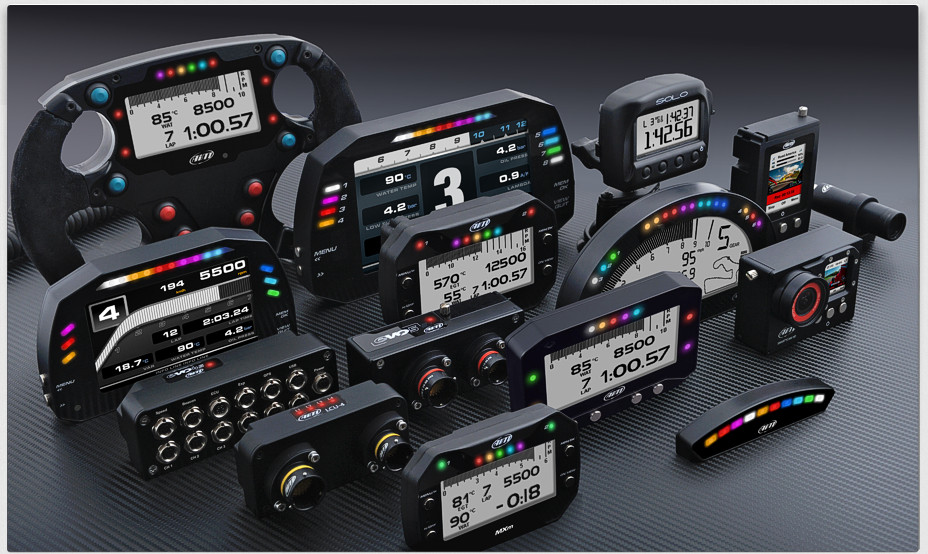
\includegraphics[width=\textwidth]{../common/images/aim-products.jpg}

    \column{0.5\textwidth}
    \begin{itemize}
    \item Embedded Linux engineer\\
      at AIM Sportline\\
      {\footnotesize\url{http://www.aim-sportline.com/}}
      \begin{itemize}
      \item Develop products on custom hardware
      \item Kernel, drivers, bootloader, FPGA
      \item Integration, build system
      \end{itemize}
    \item Open source enthusiast
      \begin{itemize}
      \item Contributor to Buildroot, the Linux kernel and a few other
        projects
      \end{itemize}
    \end{itemize}
  \end{columns}
\end{frame}


\section{Introduction}

\begin{frame}{This is not\dots}
  \begin{itemize}
  \item This is not a tutorial
  \pause
  \item This is not a feature comparison, not a selection guide
  \pause
  \item If you need one:
    \begin{itemize}
    \item Buildroot vs. OpenEmbedded/Yocto: A Four Hands
      Discussion,\\ Belloni and Petazzoni, ELC 2016
      (\href{https://elinux.org/images/7/7a/Bellonipetazzoni.pdf}{slides}
      and \href{https://www.youtube.com/watch?v=13LZ0szWSVg}{video}
      online)
    \item
      \url{http://www.jumpnowtek.com/linux/Choosing-an-embedded-linux-build-system.html}
    \item
      \url{https://opensource.com/article/18/6/embedded-linux-build-tools}
    \end{itemize}
  \pause
  \item Fact: both tools have pros and cons
  \end{itemize}
\end{frame}

\bg{both}
\begin{frame}{Similar\dots}
  \center\includegraphics[height=0.5\textheight]{images/dependencies.pdf}

  In a nutshell:\\
  a dependency graph\\
  with actions to build each node.
\end{frame}

\begin{frame}{\dots but different --- based on different tools}
  \begin{columns}
    \column{0.5\textwidth}
    \center\includegraphics[width=0.8\textwidth]{images/br-tools.pdf}
    \column{0.5\textwidth}
    \center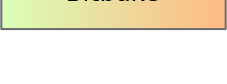
\includegraphics[width=0.8\textwidth]{images/yocto-tools.pdf}
  \end{columns}
\end{frame}

\begin{frame}{\dots but different --- root filesystem VS distribution}
  \begin{columns}
    \column{0.5\textwidth}
    \center\includegraphics[width=0.8\textwidth]{images/br-flow.pdf}
    \column{0.5\textwidth}
    \center\includegraphics[width=0.8\textwidth]{images/yocto-flow.pdf}
  \end{columns}
\end{frame}

\nobg

\begin{frame}{Topics}
  \begin{itemize}
  \item Bootstrapping
  \item Naming
  \item Writing recipes
  \item Layers / external trees
  \item Building
  \item Understanding what's going on
  \item Customizing the root filesystem
  \item Tweaking recipes
  \end{itemize}
\end{frame}


\section{Bootstrapping}


\bg{br}
\begin{frame}{Ingredients}
  \begin{itemize}
  \item Get the sources
    \begin{itemize}
    \item \texttt{git clone git://git.buildroot.net/buildroot; cd buildroot}
    \end{itemize}
  \end{itemize}
\end{frame}

\bg{yocto}
\begin{frame}{Ingredients}
  \begin{enumerate}
  \item Get the Poky sources (bitbake, oe-core)
    \begin{itemize}
    \item \texttt{git clone -b sumo git://git.yoctoproject.org/poky; cd poky}
    \end{itemize}
  \item You'll probably need more recipes
    \begin{itemize}
    \item \texttt{git clone -b sumo git://git.openembedded.org/meta-openembedded}
    \end{itemize}
  \item Additional layers can be useful
    \begin{itemize}
    \item SoC/board vendor BSP layer, additional software, \dots
    \item \url{http://layers.openembedded.org/layerindex/branch/master/layers/}
    \end{itemize}
  \end{enumerate}
\end{frame}

\bg{br}
\begin{frame}{Configure}
  \begin{itemize}
  \item Smooth start: find a defconfig for a similar board
    \begin{itemize}
    \item \texttt{make list-defconfigs \ \ \ \ \ \ \ \ \# minimal booting configs}
    \item \texttt{make similar\_board\_defconfig}
    \end{itemize}
  \item Or from scratch
    \begin{itemize}
    \item Find kernel and U-Boot sources that work for your SoC
    \item \texttt{make menuconfig}
      \begin{itemize}
      \item Target: architecture, CPU features
      \item Kernel: where to fetch it from, defconfig, dtbs
      \item U-Boot: where to fetch it from, defconfig
      \end{itemize}
    \end{itemize}
  \end{itemize}
\end{frame}

\begin{frame}
  \center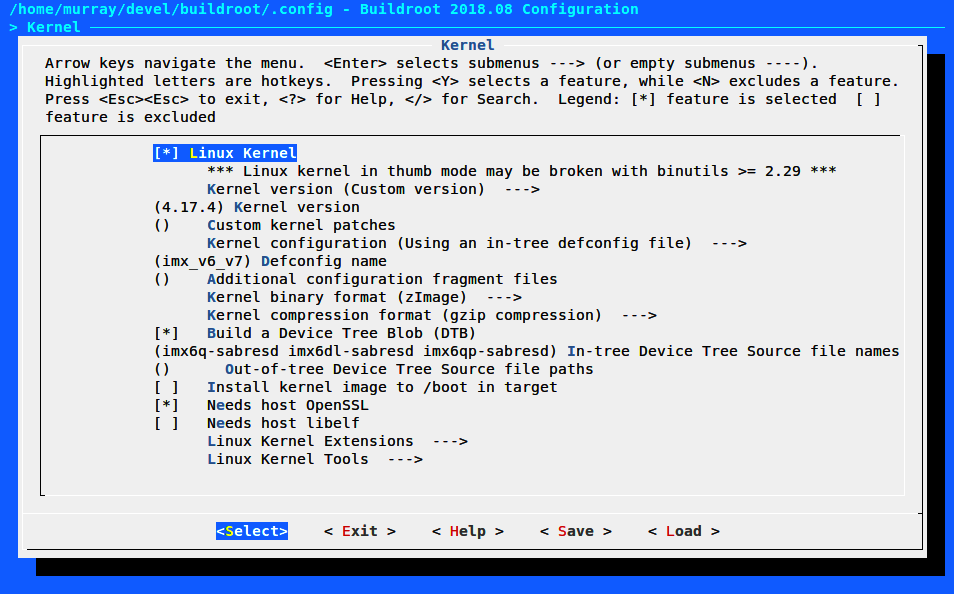
\includegraphics[height=1.0\textheight]{images/br-menuconfig-kernel.png}
\end{frame}

\bg{yocto}
\begin{frame}[fragile]{Configure}
  \begin{itemize}
  \item {\tt . oe-init-build-env \ \ \ \ \ \# creates and enters the build/ dir}
  \item Smooth start: find a defconfig for a similar board
    \begin{itemize}
    \item {\tt ls conf/machine/} in your SoC vendor layer
    \item Set {\tt MACHINE ?= "<similar\_machine>"} in {\tt conf/local.conf}
    \end{itemize}
  \end{itemize}
\end{frame}

\bg{br}
\begin{frame}[fragile]{Build}
  \begin{itemize}
  \item {\tt make}
    \begin{itemize}
    \item Without parameters builds ``all''
    \end{itemize}
  \end{itemize}
\end{frame}

\bg{yocto}
\begin{frame}[fragile]{Build}
  \begin{itemize}
  \item {\tt bitbake <IMAGE>}
  \item {\tt bitbake core-image-minimal}
  \end{itemize}
\end{frame}

\nobg


\section{Naming}


\begin{frame}{Building items}
  \center\includegraphics[height=0.7\textheight]{images/dependencies2.pdf}
\end{frame}


\bg{both}
\begin{frame}{Package == Recipe}
  \begin{center}
    Rules to download and ``build'' a single program, library or other\\
    (e.g. binutils, busybox, gcc, libxml2)
  \end{center}

  \begin{columns}
    \column{0.5\textwidth}
    \begin{itemize}
    \item Each package is a Make target\\
      and has a Kconfig on/off knob
    \item {\tt make libxml2}
    \item {\tt host-<PKG>}: the same package built for the development
      host (native build)
    \end{itemize}

    \column{0.5\textwidth}
    \begin{itemize}
    \item Each package is a Bitbake target\\
      {\ } % to keep bullets aligned
    \item {\tt bitbake libxml2}
    \item {\tt <PKG>-native}: the same package built for the
      development host (native build)
    \end{itemize}
  \end{columns}
\end{frame}

\begin{frame}{Step == Task}
  \begin{center}
    Each package requires several steps to be built
  \end{center}

  \begin{columns}
    \column{0.5\textwidth}
    \begin{itemize}
    \item No formal name, usually called just {\em steps}
    \item {\tt source}, {\tt extract}, {\tt patch}, {\tt configure},
      {\tt build}, {\tt install}, \dots
    \item Each step is also a make target
    \item The special {\tt <PKGNAME>} make target depends on all other normal
      tasks required to 'build' a recipe
    \item {\tt make libxml2-configure host-binutils-build busybox}
    \end{itemize}

    \column{0.5\textwidth}
    \begin{itemize}
    \item Called {\em tasks}\\
      (often prefixed with {\tt do\_})
    \item {\tt fetch}, {\tt unpack}, {\tt patch}, {\tt configure},
      {\tt compile}, {\tt install}, {\tt deploy}, \dots
    \item First-class citizens in bitbake
    \item The special {\tt build} task depends on all other normal
      tasks required to 'build' a recipe
    \item {\tt bitbake -c configure\\
      libxml2 busybox}
    \end{itemize}
  \end{columns}
\end{frame}

\begin{frame}{Default steps/tasks}
  \begin{columns}
    \column{0.5\textwidth}
    \center\includegraphics[height=0.95\textheight]{images/br-steps.pdf}
    \column{0.5\textwidth}
  \center\includegraphics[height=0.95\textheight]{images/yocto-tasks.pdf}
  \end{columns}
\end{frame}

\begin{frame}{Naming side-by-side}
  \begin{table}
    \begin{tabular}{cc}
      \toprule
      Package & Recipe\\
      Package Step & Recipe Task\\
      {\tt host-<PKG>} & {\tt <PKG>-native}\\
      \midrule
      {\tt pkg-generic.mk} & {\tt base.bbclass}\\
      \midrule
      source                      & fetch\\
      extract                     & unpack\\
      patch                       & patch\\
      configure                   & configure\\
      build                       & compile\\
      install-\{target,staging\}  & install\\
      install-images              & deploy\\
      \bottomrule
    \end{tabular}
  \end{table}
\end{frame}

\nobg


\section{Layers / external trees}


\bg{yocto}

\bg{yocto}
\begin{frame}[fragile]{Yocto: layers}
  The preferred way to add features: layers
  
  {\tt conf/bblayers.conf}
  \begin{minted}[frame=single,autogobble,fontsize=\small]{diff}
   BBLAYERS ?= " \
     /home/murray/devel/poky/meta \
     /home/murray/devel/poky/meta-poky \
     /home/murray/devel/poky/meta-yocto-bsp \
     <...path to other layers...> \
     "
  \end{minted}
\end{frame}

\begin{frame}[fragile]{Yocto: adding layers}
  \begin{minted}[frame=single,autogobble,fontsize=\small]{diff}
   BBLAYERS ?= " \
     /home/murray/devel/poky/meta \
     /home/murray/devel/poky/meta-poky \
     /home/murray/devel/poky/meta-yocto-bsp \
  +  ${TOPDIR}/../meta-my-soc-vendor \
  +  ${TOPDIR}/../meta-openembedded/meta-oe \
     "
  \end{minted}

  \begin{itemize}
  \item Suggestion: use relative paths
  \end{itemize}
\end{frame}

\begin{frame}{Yocto: {\tt .bbappend}}
  \begin{itemize}
  \item {\tt .bbappend} files are appended to the {\tt .bb} file while
    parsing
    \begin{itemize}
    \item Change variable values
    \item Append/prepend to tasks
    \end{itemize}
  \item The resulting {\tt myrecipe} is a concatenation of:
    \begin{itemize}
    \item {\tt <LAYER1>/*/*/myrecipe.bb}
    \item {\tt <LAYER2>/*/*/myrecipe.bbappend}
    \item {\tt <LAYER3>/*/*/myrecipe.bbappend}
    \end{itemize}
  \end{itemize}
\end{frame}

\begin{frame}[fragile]{Yocto: issues with layers}
  \begin{itemize}
  \item Some SoC vendor layers augment the buildsystem, at times
    creating problems
  \item Conflict between layers (e.g. in gstreamer)
  \item Suggestion: add layers one by one, bottom-up, test each time
  \item Problems?
    \begin{itemize}
    \item Fix the offending code in your layer ({\tt .bbappend})
    \item disable the recipe ({\tt PNBLACKLIST}) and provide an alternative
    \item Don't use the layer, copy only what you need
    \end{itemize}
  \end{itemize}
\end{frame}

\begin{frame}[fragile]{Yocto: your top-level layer}
  \begin{itemize}
  \item Add your top-level layer
    \begin{itemize}
    \item Your machine configuration
    \item Your proprietary packages
    \item {\tt .bbappends} and other files to modify the behaviour of
      lower layers
    \end{itemize}
\end{itemize}
\end{frame}

\bg{br}
\begin{frame}{Buildroot: {\tt BR2\_EXTERNAL}}
  \begin{itemize}
  \item {\tt BR2\_EXTERNAL} is technically similar to Yocto layers,
    but simpler
  \item The goal is to add, not modify
  \item Typical use: add your own product customizations
    \begin{itemize}
    \item packages
    \item Kconfig options
    \item defconfigs
    \item boards
    \item patches
    \item \dots
    \end{itemize}
  \item Need to fix/improve a Buildroot package?
    \begin{itemize}
    \item Suggested policy: do it in the Buildroot code, then submit
      your improvements upstream
    \end{itemize}
  \end{itemize}
\end{frame}

\begin{frame}[fragile]{Buildroot: {\tt BR2\_EXTERNAL}}
  \begin{minted}[frame=single,autogobble,fontsize=\small]{shell-session}
    $ make BR2_EXTERNAL=~/devel/myext:~/devel/myext2 menuconfig
  \end{minted}

  \begin{itemize}
  \item The list of your externals is saved internally ({\tt .output/.br-external.mk})
  \item The top-level Makefile will include each external Makefile
  \item The same for Config.in files
  \end{itemize}
\end{frame}

\nobg


\section{Writing recipes}


\bg{yocto}
\begin{frame}[fragile]{A simple Yocto package: the {\tt .bb} file}

  {\tt <MYLAYER>/recipes-app/corporate-apps/foo\_1.0.bb}
  \begin{minted}[frame=single,autogobble,fontsize=\footnotesize]{bash}
    SRC_URI = "http://www.foo.org/download/foo-${PV}.tar.xz"
    DEPENDS = "libbar-native libusb"

    do_compile() {
        oe_runmake all
    }

    do_install() {
        install -D -m 0755 ${B}/foo ${D}${bindir}/foo
    }
  \end{minted}
\end{frame}

\bg{br}
\begin{frame}[fragile]{A simple Buildroot package: the makefile}

  {\tt package/foo/foo.mk}
  \begin{minted}[frame=single,autogobble,fontsize=\footnotesize]{makefile}
    FOO_VERSION = 1.0
    FOO_SITE = http://www.foo.org/download
    FOO_DEPENDENCIES = host-libbar libusb

    define FOO_BUILD_CMDS
        $(MAKE) $(TARGET_CONFIGURE_OPTS) -C $(@D) all
    endef

    define FOO_INSTALL_TARGET_CMDS
        $(INSTALL) -D -m 0755 $(@D)/foo $(TARGET_DIR)/usr/bin/foo
    endef

    $(eval $(generic-package))
  \end{minted}
\end{frame}

\begin{frame}[fragile]{A simple Buildroot package: {\tt Config.in}}
  \begin{itemize}
  \item Shows the package in the Kconfig interfaces
  \item Uses the Kconfig language
  \end{itemize}
  {\tt package/foo/Config.in}
  \begin{minted}[frame=single,autogobble,fontsize=\footnotesize]{Kconfig}
    config BR2_PACKAGE_FOO
            bool "foo"
            select BR2_PACKAGE_LIBUSB
            help
              A brief description.
  \end{minted}
\end{frame}

\bg{yocto}
\begin{frame}[fragile]{Yocto classes}
  \begin{itemize}
  \item {\em classes} implement common features for reuse in recipes
    \begin{itemize}
    \item {\tt .bbclass} files
     \item There are classes for the most common build tools:
      Autotools, CMake
    \end{itemize}
  \end{itemize}
  {\tt <MYLAYER>/recipes-app/corporate-apps/foo\_1.0.bb}
  \begin{minted}[frame=single,autogobble,fontsize=\footnotesize]{bash}
    SRC_URI = "http://www.foo.org/download/foo-${PV}.tar.xz"
    DEPENDS = "libbar-native libusb"

    inherit autotools
  \end{minted}
\end{frame}

\bg{br}
\begin{frame}[fragile]{Buildroot package infrastructures}
  \begin{itemize}
  \item {\em package infrastructures} are classes of packages that use the same build tool
    \begin{itemize}
    \item Autotools, CMake, Python, LuaRocks, Perl/CPAN \dots
    \end{itemize}
  \item Most commands have a default
  \end{itemize}
  {\tt package/foo/foo.mk}
  \begin{minted}[frame=single,autogobble,fontsize=\footnotesize]{makefile}
    FOO_VERSION = 1.0
    FOO_SITE = http://www.foo.org/download
    FOO_DEPENDENCIES = host-libbar libusb

    $(eval $(autotools-package))
  \end{minted}
\end{frame}

\bg{yocto}
\begin{frame}[fragile]{Yocto classes}
  \begin{itemize}
  \item With classes the common {\tt do\_<TASK>} functions are already
    set
  \item Customizable via infrastructure-specific variables
    \begin{minted}[autogobble,fontsize=\footnotesize]{bash}
      EXTRA_OECONF += "--enable-warp-speed"
    \end{minted}
  \item Can be extended with
    \begin{itemize}
    \item {\tt do\_<TASK>\_prepend}
    \item {\tt do\_<TASK>\_append}
      \begin{minted}[autogobble,fontsize=\footnotesize]{bash}
        do_install_append() {
            touch ${D}${sysconfdir}/foo.conf
        }
      \end{minted}
    \end{itemize}
  \end{itemize}
\end{frame}

\bg{br}
\begin{frame}[fragile]{Buildroot package infrastructures}
  \begin{itemize}
  \item With package infrastructures {\tt FOO\_<STEP>\_CMDS} are already set
  \item Customizable via infrastructure-specific variables
    \begin{minted}[autogobble,fontsize=\footnotesize]{makefile}
      FOO_CONF_OPTS = --enable-warp-speed
    \end{minted}
  \item To extend them define hooks
    \begin{itemize}
    \item {\tt FOO\_PRE\_<STEP>\_HOOKS}
    \item {\tt FOO\_POST\_<STEP>\_HOOKS}
      \begin{minted}[autogobble,fontsize=\footnotesize]{makefile}
        define FOO_CREATE_CONF_FILE
            touch $(TARGET_DIR)/etc/foo.conf
        endef
        FOO_POST_INSTALL_HOOKS += FOO_CREATE_CONF_FILE
      \end{minted}
    \end{itemize}
  \end{itemize}
\end{frame}

\bg{both}
\begin{frame}{Predefined variables}
  Lots of predefined variables can (and should) be user in rules. The
  most widely used:
  \begin{table}
    \begin{tabular}{lll}
      \toprule
      & Buildroot & Yocto\\
      \midrule
      Package name          & {\tt <PKG>\_NAME}              & {\tt PN}\\
      Package raw name      & {\tt <PKG>\_RAWNAME}           & {\tt BPN}\\
      Package version       & {\tt <PKG>\_VERSION}           & {\tt PV}\\
      \midrule
      Source code dir       & {\tt <PKG>\_SRCDIR}            & {\tt S}\\
      Build dir             & {\tt <PKG>\_BUILDDIR}          & {\tt B}\\
      Install files in (*)  & {\tt TARGET\_DIR}              & {\tt D}\\
      Install images in (*) & {\tt BINARIES\_DIR}            & {\tt DEPLOYDIR}\\
      \bottomrule
    \end{tabular}
  \end{table}
  \begin{itemize}
  \item[*] The final dirs in Buildroot, temp dirs in Yocto.
  \end{itemize}
\end{frame}

\bg{both}

\begin{frame}{Adding patches}
  \begin{table}
    \begin{tabular}{cc}
      \toprule
      Buildroot & Yocto\\
      \midrule
      {\tt .patch} file in package dir   & {\tt .patch} file in recipe subdir (*)\\
      {\tt <PKG>\_PATCH = <URL>}         & {\tt SRC\_URI += <URL>}\\
      {\tt BR2\_GLOBAL\_PATCH\_DIR} tree & Your layer\\
      \bottomrule
    \end{tabular}
  \end{table}
  \begin{itemize}
  \item[*] Plus {\tt SRC\_URI += "file://foo.patch"} \\
    (and {\tt FILESEXTRAPATHS\_prepend = "<DIR>:"})
  \end{itemize}
\end{frame}

\begin{frame}{Overall recipe directory layout}
  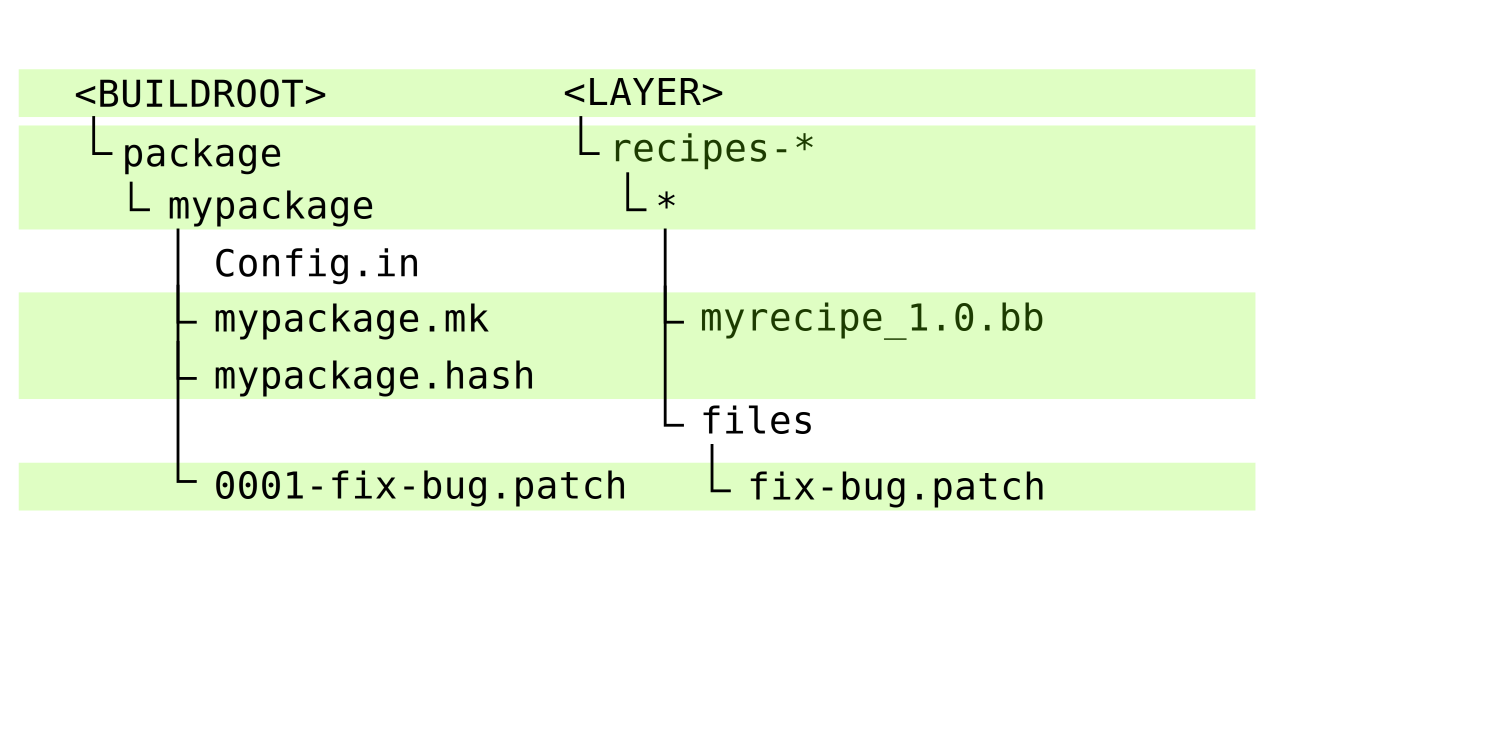
\includegraphics[width=0.9\textwidth]{images/recipe-dirs-layout.pdf}
\end{frame}

\nobg


\section{Building}


\bg{both}
\begin{frame}{Invoking}
  \begin{table}
    \begin{tabular}{ll}
      \toprule
      Buildroot & Yocto\\
      \midrule
      {\tt make} {\tt \textcolor{gray}{[all]}}
                                     & {\tt bitbake <IMAGE>}\\
      {\tt make busybox}             & {\tt bitbake busybox}\\
      {\tt make busybox-configure}   & {\tt bitbake -c configure busybox}\\
      \midrule
      {\tt make busybox-reconfigure} & {\tt bitbake -C configure busybox}\\
      \midrule
      {\tt make clean}               & {\tt bitbake -c clean world}\\
      {\tt make busybox-dirclean}    & {\tt bitbake -c clean busybox}\\
      \bottomrule
    \end{tabular}
  \end{table}
\end{frame}

\begin{frame}{Tuning resource usage}
  \begin{table}
    \begin{tabular}{ll}
      \toprule
      Buildroot & Yocto\\
      \midrule
      {\tt BR2\_JLEVEL=2 make}       & {\tt PARALLEL\_MAKE="-j 2" bitbake ...}\\
      ---                            & {\tt BB\_NUMBER\_THREADS=2 bitbake ...}\\
      {\tt Build options \textrightarrow{} Enable compiler cache} & ---\\
      ---                            & {\tt SSTATE\_DIR ?= "~/.sstate-cache"}\\
      \bottomrule
    \end{tabular}
  \end{table}
\end{frame}

\bg{br}
\begin{frame}{Buildroot: out-of-tree builds}
  \begin{itemize}
  \item {\tt make O=foo foo\_defconfig}
  \item {\tt make O=bar bar\_defconfig}
  \item {\tt cd foo; make}
    \begin{itemize}
    \item Build in {\tt foo/*} instead of {\tt output/*}
    \end{itemize}
  \pause
  \item {\tt cd bar; make}
    \begin{itemize}
    \item Can run in parallel
    \end{itemize}
  \end{itemize}
\end{frame}

\bg{yocto}
\begin{frame}{Yocto: multiple machines and images}
  \begin{itemize}
  \item {\tt bitbake core-image-minimal}
  \item {\tt bitbake my-image-huge}
    \begin{itemize}
    \item Recycles common artifacts
    \end{itemize}
  \pause
  \item {\tt MACHINE=another-board bitbake my-image-huge}
    \begin{itemize}
    \item Remember to use {\tt ?=} to set {\tt MACHINE} in your conf
      file
    \end{itemize}
  \end{itemize}
\end{frame}

\bg{br}
\begin{frame}{Buildroot dependency tracking: stamp files}
  \begin{itemize}
  \item Dependency tracking is at the core of Make
    (program \textrightarrow{} .o \textrightarrow{} .c)
    \begin{itemize}
    \item Does not fit completely the needs of a buildsystem
    \end{itemize}
  \item Internally Buildroot touches a {\em stamp file} after
    completing each step
    \begin{itemize}
    \item An empty file
    \item Tracks successful step completion, not the rules that originated it
    \item If the rules change, Buildroot is unaware
    \end{itemize}
  \end{itemize}
\end{frame}

\begin{frame}{Buildroot dependency tracking: stamp files}
  \begin{itemize}
  \item You need to manually trigger a rebuild when:
    \begin{itemize}
    \item You changed the configuation of the package or one of its dependencies
    \item You're developing the package and changed the rules ({\tt .mk}, patches\dots)
    \end{itemize}
  \item How to rebuild
    \begin{itemize}
    \item The safe option: {\tt make clean; make}
    \item If you know what you really need: {\tt make <PKG>-dirclean <PKG>}
    \item Or {\tt make <PKG>-reconfigure} / {\tt make <PKG>-rebuild}
    \end{itemize}
  \end{itemize}
\end{frame}

\bg{yocto}
\begin{frame}{Yocto: recipe hash}
  \begin{itemize}
  \item Bitbake stores a hash for each task
  \item Hash content:
    \begin{itemize}
    \item All the recipe variables and task code ({\tt bitbake -e})
    \item Content of all files stored in {\tt SRC\_URI}
    \end{itemize}
  \item Automatically detect recipe changes and rebuilds what's needed
  \item Result stores in the {\em sstate cache} for later reuse
  \end{itemize}
\end{frame}

\begin{frame}{Yocto: recipe hash}
  \begin{itemize}
  \item Still want to force a task?
    \begin{itemize}
    \item {\tt bitbake -f -c configure <PKG>}
    \item {\tt -f} forces to run tasks even when not needed
    \end{itemize}
  \end{itemize}
\end{frame}

\bg{standout}
\begin{frame}[standout]
  Where are my output files?
\end{frame}

\bg{both}
\begin{frame}{Work directory layout}
  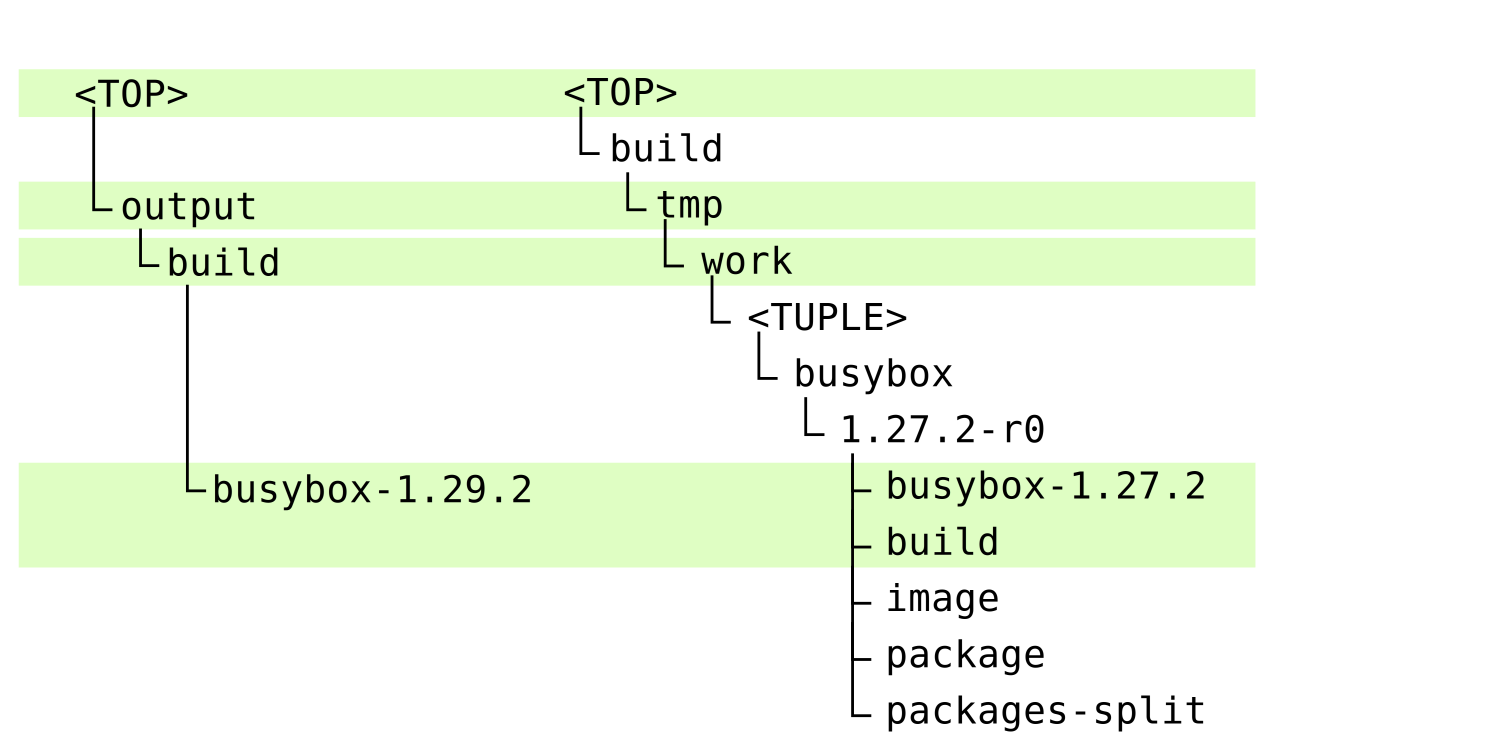
\includegraphics[width=0.9\textwidth]{images/out-dirs-build.pdf}
\end{frame}

\begin{frame}{Root filesystem generation}
  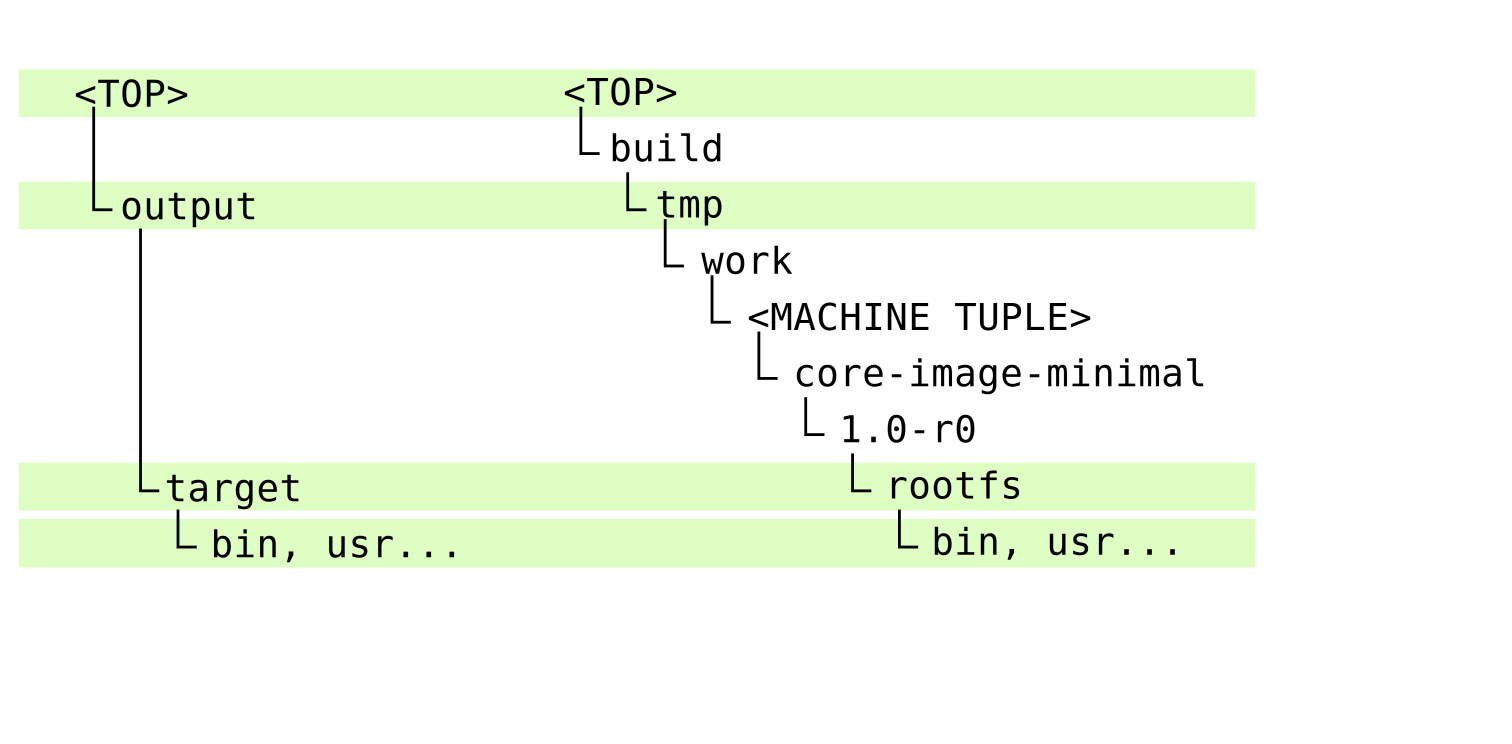
\includegraphics[width=0.9\textwidth]{images/out-dirs-rootfs.pdf}
\end{frame}

\begin{frame}{Output directory layout}
  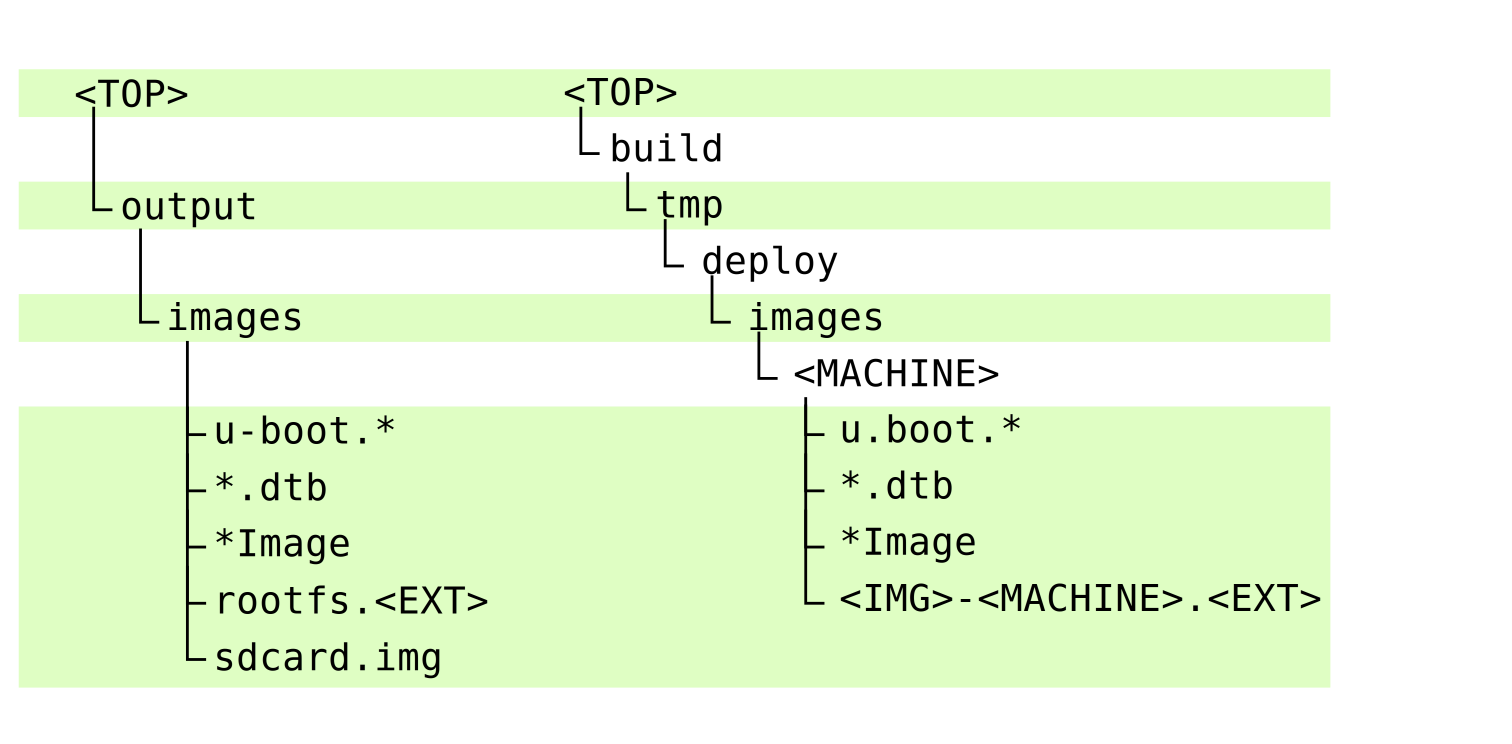
\includegraphics[width=0.9\textwidth]{images/out-dirs-images.pdf}
\end{frame}

\nobg


\section{Understanding what's going on}


\bg{standout}
\begin{frame}[standout]
  What will it build?
\end{frame}

\bg{br}
\begin{frame}{Buildroot: {\tt graph-depends}}
  \begin{itemize}
  \item {\tt make graph-depends}
  \item Produces {\tt output/graphs/graph-depends.pdf}
  \end{itemize}
  \center\includegraphics[height=0.75\textheight]{images/br-graph-depends.pdf}
\end{frame}

\begin{frame}{Buildroot: {\tt graph-depends}}
  \begin{itemize}
  \item Build a per-package graph: {\tt <PKG>-graph-depends}
  \item Set {\tt BR2\_GRAPH\_DEPS\_OPTS} in the environment to control
    the output
  \item {\tt BR2\_GRAPH\_DEPS\_OPTS="--exclude=host" make avahi-graph-depends}
  \item Produces {\tt output/graphs/avahi-graph-depends.pdf}
  \end{itemize}
  \center\includegraphics[height=0.65\textheight]{images/br-avahi-graph-depends.pdf}
\end{frame}

\bg{yocto}
\begin{frame}{Yocto: {\tt taskexp}}
  \begin{itemize}
  \item Generating dot graphs not really usable
  \item Task Explorer: {\tt bitbake -g -u taskexp world}
  \item Shows dependencies between tasks (not recipes)
  \end{itemize}
  \center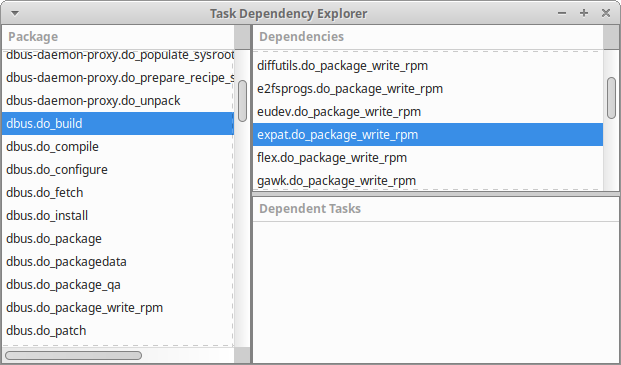
\includegraphics[height=0.65\textheight]{images/yocto-taskexp.png}
\end{frame}

\bg{standout}
\begin{frame}[standout]
  What does it do?

  What went wrong?
\end{frame}

\bg{br}
\begin{frame}[fragile]{Buildroot: default output}
  \begin{minted}[frame=single,autogobble,fontsize=\small]{shell-session}
    $ make
    ...
    >>> host-e2fsprogs 1.44.2 Extracting
    xzcat /home/murray/src/e2fsprogs/e2fsprogs-1.44.2.tar.xz...
    >>> host-e2fsprogs 1.44.2 Patching
    >>> host-e2fsprogs 1.44.2 Configuring
    checking build system type... x86_64-pc-linux-gnu
    checking host system type... x86_64-pc-linux-gnu
    ...
  \end{minted}
  \begin{itemize}
  \item ``{\tt >>>}'' marks the started tasks
  \item The whole output of each step follows
  \item Failure? Look at the last lines
  \end{itemize}
\end{frame}

\begin{frame}[fragile]{Buildroot: concise output}
  \begin{minted}[frame=single,autogobble,fontsize=\small]{shell-session}
    $ ./utils/brmake
    ...
    2018-10-06T16:15:58 >>> host-zlib  Patching
    2018-10-06T16:15:58 >>> host-zlib  Configuring
    2018-10-06T16:15:58 >>> host-zlib  Building
    2018-10-06T16:15:58 >>> host-zlib  Installing to host directory
    2018-10-06T16:15:58 >>> host-util-linux 2.32.1 Patching
    ...
  \end{minted}
  \begin{itemize}
  \item Adds step start time
  \item Verbose output saved in {\tt br.log}
  \end{itemize}
\end{frame}

\bg{yocto}
\begin{frame}[fragile]{Yocto: default output}
  \begin{itemize}
  \item The default output shows the current status, no logs
  \item Hides completed tasks
  \end{itemize}
  \begin{minted}[frame=single,autogobble,fontsize=\footnotesize]{shell-session}
    Currently  4 running tasks (119 of 2503)   4% |##                              |
    0: glibc-initial-2.27-r0 do_fetch (pid 5216)  38% |############        | 4.09M/s
    1: glibc-2.27-r0 do_fetch - 4s (pid 5261)
    2: ncurses-native-6.0+20171125-r0 do_fetch (pid 6147) |            <=>         |
    3: elfutils-native-0.170-r0 do_fetch (pid 7143)  11% |###              | 2.49M/s
  \end{minted}
\end{frame}

\begin{frame}[fragile]{Yocto: concise ``log'' output}
  \begin{itemize}
  \item To see the completed tasks:
  \item {\tt bitbake ... | cat}
  \end{itemize}
  \begin{minted}[frame=single,autogobble,fontsize=\footnotesize]{shell-session}
    NOTE: Running task 119 of 2645 (.../binutils/binutils-cross_2.30.bb:do_unpack)
    NOTE: Running task 232 of 2645 (virtual:native:...lzo/lzo_2.10.bb:do_compile)
    NOTE: recipe binutils-cross-arm-2.30-r0: task do_unpack: Started
    NOTE: recipe binutils-cross-arm-2.30-r0: task do_prepare_recipe_sysroot: Started
    NOTE: recipe elfutils-native-0.170-r0: task do_prepare_recipe_sysroot: Started
    NOTE: recipe lzo-native-2.10-r0: task do_compile: Started
    NOTE: recipe elfutils-native-0.170-r0: task do_prepare_recipe_sysroot: Succeeded
    NOTE: Running task 247 of 2645 (virtual:native:.../elfutils_0.170.bb:do_configure)
    NOTE: recipe binutils-cross-arm-2.30-r0: task do_prepare_recipe_sysroot: Succeeded
  \end{minted}
\end{frame}

\begin{frame}{Yocto: inspect build logs}
  \begin{itemize}
  \item Failure?
  \item For each task a log file is saved
    \begin{itemize}
    \item in {\tt tmp/work/<TUPLE>/<RECIPE>/<VERSION>/temp/log.do\_<TASK>}
    \item e.g. {\tt tmp/work/x86\_64-linux/gmp-native/6.1.2-r0/temp/log.do\_configure}
    \end{itemize}
  \item Or re-run the failed task with verbose output to see its
    output on your terminal
    \begin{itemize}
    \item {\tt bitbake -v -f -c configure gmp-native}
    \end{itemize}
  \end{itemize}
\end{frame}

\bg{standout}
\begin{frame}[standout]
  What is it thinking?
\end{frame}

\bg{br}
\begin{frame}{Buildroot: {\tt printvars}}
  \begin{itemize}
  \item {\tt make -s printvars}
    \begin{itemize}
    \item Print all variables
    \end{itemize}
  \item {\tt make -s VARS=BUSYBOX\_\% printvars}
    \begin{itemize}
    \item Only variables matching a pattern
    \end{itemize}
  \item {\tt make -s RAW\_VARS=YES printvars}
    \begin{itemize}
    \item Print unexpanded values
    \end{itemize}
  \item {\tt make -qp}
    \begin{itemize}
      \item Print the whole Make database
      \item Variables (before expansion) and the file where they were
        set
      \item Rules (target + prerequisites + actions)
    \end{itemize}
  \end{itemize}
\end{frame}

\bg{yocto}
\begin{frame}{Yocto: {\tt bitbake -e}}
  \begin{itemize}
  \item {\tt bitbake -e}
    \begin{itemize}
    \item Show the global environment
    \item Variables and the files where they were set
    \end{itemize}
  \item {\tt bitbake -e <RECIPE>}
    \begin{itemize}
    \item Show the per-recipe environment
    \item Variables and the files where they were set
    \item Tasks actions
    \end{itemize}
  \end{itemize}
\end{frame}

\nobg


\section{Customizing the root filesystem}


\bg{br}
\begin{frame}{Buildroot: Kconfig}
  \begin{itemize}
  \item The same configuration system as the kernel, Busybox, U-Boot,
    Barebox\dots
  \item {\tt make menuconfig}, {\tt make xconfig}
  \item {\tt .config} is your current configuration
  \item {\tt make savedefconfig} updates your defconfig with the new
    values
  \end{itemize}
\end{frame}

\bg{yocto}
\begin{frame}{Yocto: {\tt .bb} files}
  \begin{itemize}
  \item Your ``configuration'' is in several {\tt .bb} files.
  \item A common layout:
    \begin{itemize}
    \item Build options, toolchain, {\tt MACHINE}: a conf file in your
      top layer \\
      (or {\tt build/conf/local.conf})
    \item Target options, kernel and bootloader selection: in your
      layer {\tt conf/machine/<MACHINE>.bb}
    \item System configuration: various recipes, other places
    \item Packages to put in rootfs: image recipe (see later)
    \end{itemize}
  \end{itemize}
\end{frame}

\bg{br}
\begin{frame}{Buildroot: adding packages}
  \begin{itemize}
  \item {\tt make menuconfig} \textrightarrow{} Packages
    \begin{itemize}
    \item Search, add, remove, change packages
      \end{itemize}
  \item {\tt make clean} (if you changed or remove packages)
  \item {\tt make}
  \end{itemize}
\end{frame}

\bg{yocto}
\begin{frame}[fragile]{Yocto: adding packages}
  \begin{itemize}
  \item Find the package you need
    \begin{itemize}
    \item {\tt bitbake-layers show-recipes}
    \item \url{http://layers.openembedded.org/layerindex/branch/master/layers/}
    \end{itemize}
  \item Create your own image recipe
    \begin{itemize}
    \item Image = list of packages to but in rootfs (a subset of all
      the packages)
    \end{itemize}
  \end{itemize}
\end{frame}

\begin{frame}[fragile]{Yocto: adding packages}
  \begin{itemize}
  \item Create an image recipe ({\tt <MYLAYER>/recipes-*/images/*-image-*.bb})
    \begin{minted}[frame=single,autogobble,fontsize=\footnotesize]{bash}
      require recipes-core/images/core-image-minimal.bb
      DESCRIPTION = "My own root filesystem"
      LICENSE = "MIT"
      IMAGE_FSTYPES = "tar.gz"
      IMAGE_INSTALL += "htop packagegroup-debug"
    \end{minted}
  \item Package groups ({\tt
    <MYLAYER>/recipes-*/packagegroups/packagegroup-*.bb})
    \begin{minted}[frame=single,autogobble,fontsize=\footnotesize]{bash}
      inherit packagegroup
      RDEPENDS_${PN} = "gdb strace"
    \end{minted}
  \end{itemize}
\end{frame}

\bg{both}
\begin{frame}{Typical root filesystem customizations}
  \begin{itemize}
  \item And embedded systems needs customizations
    \begin{itemize}
    \item High-level choices: init system, /dev management, locales\dots
    \item Creation of users, passwords, assorted files, \dots
    \item And many more
    \end{itemize}
  \item Buildroot
    \begin{itemize}
    \item {\tt make menuconfig} \textrightarrow{} {\tt System
      configuration}
    \end{itemize}
  \item Yocto
    \begin{itemize}
    \item Add appropriate lines to your conf, board or image files
    \item Search the Yocto reference manual
      \url{https://www.yoctoproject.org/docs/current/ref-manual/ref-manual.html}
    \item Grep the poky source code
    \end{itemize}
  \end{itemize}
\end{frame}

\begin{frame}{Some system settings, side-by-side}
  \begin{table}
    \begin{tabular}{ll}
      \toprule
      Buildroot & Yocto\\
      \midrule
      {\tt System hostname} & {\tt hostname\_pn-base-files = "mybox"}\\
      {\tt System banner}   & {\tt DISTRO\_NAME\_pn-base-files = "Welcome"},\\
                            & {\tt DISTRO\_VERSION\_pn-base-files = ""}\\
      \midrule
      {\tt Init system}     & {\tt VIRTUAL-RUNTIME\_init\_manager}\\
      {\tt /dev management} & {\tt VIRTUAL-RUNTIME\_dev\_manager}\\
      \midrule
      {\tt Root password} & {\tt IMAGE\_FEATURES += "empty-root-password"}\\
      {\tt Users tables} & {\tt inherit extrausers;}\\
                         & {\tt EXTRA\_USERS\_PARAMS = "usermod -P 1876*18 root;"}\\
      \bottomrule
    \end{tabular}
  \end{table}
\end{frame}

\begin{frame}{Other rootfs customizations}
  \begin{itemize}
  \item Buildroot: {\tt System configuration} menu:
    \begin{itemize}
    \item Root filesystem overlay directories
    \item Post-build and post-image scripts
    \end{itemize}
  \item Yocto
    \begin{itemize}
    \item {\tt ROOTFS\_POSTPROCESS\_COMMAND} and {\tt
      IMAGE\_POSTPROCESS\_COMMAND}
    \end{itemize}
  \end{itemize}
\end{frame}

\nobg


\section{Tweaking recipes}


\bg{both}
\begin{frame}{Configuring Kconfig-based packages}
  \begin{itemize}
  \item Buildroot
    \begin{itemize}
    \item Based on {\tt kconfig-package}
    \item Kconfig packages: at91bootstrap3, barebox, uboot, linux,
      busybox, linux-backports, swupdate, uclibc, xvisor
    \end{itemize}
  \item Yocto
    \begin{itemize}
    \item Inherit the obscure {\tt cml1} class
    \item Kconfig packages in the Poky layer: linux, busybox (not
      U-Boot)
    \end{itemize}
  \end{itemize}
\end{frame}

\begin{frame}{Configuring Kconfig-based packages}
  \small
  \begin{table}
    \begin{tabular}{lll}
      \toprule
      Description & Buildroot & Yocto\\
      \midrule
      Enter menu       & {\tt make <PKG>-menuconfig}       & {\tt bitbake -c menuconfig <RCP>}\\
      \midrule
      Save defconfig   & {\tt make <PKG>-savedefconfig}    & {\tt bitbake -c savedefconfig <RCP>}\\
      Update defconfig & {\tt make <PKG>-update-defconfig} & ---\\
      Extract fragment & ---                               & {\tt bitbake -c diffconfig <RCP>}\\
      \bottomrule
    \end{tabular}
  \end{table}
\end{frame}

\bg{yocto}
\begin{frame}{Yocto: (re)assigning variables}
  \begin{itemize}
  \item Assignments
    \begin{itemize}
    \item {\tt F := "foo-\$\{A\}"} --- Immediate expansion
    \item {\tt F = "foo-\$\{A\}"} --- Expansion on usage
    \end{itemize}
  \item Weak assignments: used for values the user is supposed to customize
    \begin{itemize}
    \item Base layer {\tt .bb}: {\tt VAR ??= "white"}
    \item Middle layer {\tt .bbappend}: {\tt VAR ?= "black"}
    \item Top-level layer{\tt .bbappend}: {\tt VAR = "green"}
    \item The recipe will use {\tt VAR = "green"}
    \end{itemize}
  \item Append or prepend
    \begin{itemize}
    \item {\tt VAR += "val"}, {\tt VAR =+ "val"} (adds spaces)
    \item {\tt VAR\_append = "val"}, {\tt VAR\_prepend = "val"} (does not add spaces)
    \item {\tt VAR\_remove = "val"}
    \end{itemize}
  \end{itemize}
\end{frame}

\bg{br}
\begin{frame}{Buildroot: (re)assigning variables}
  \begin{itemize}
  \item It's a Makefile, use the Make syntax
  \item Assignments
    \begin{itemize}
    \item {\tt F := "foo-\$(VER)"} --- Immediate expansion
    \item {\tt F = "foo-\$(VER)"} --- Expansion on usage
    \end{itemize}
  \item Append or prepend
    \begin{itemize}
    \item {\tt VAR = "\$(VAR) extra"}, {\tt VAR = "extra \$(VAR)"}
    \end{itemize}
  \end{itemize}
\end{frame}

\bg{both}
\begin{frame}{More string processing}
  \begin{itemize}
  \item Buildroot
    \begin{itemize}
    \item Make has several functions for transforming text
    \item Example: {\tt VAR = \$(filter-out bug, foo bug bar)}
    \end{itemize}
  \item Yocto
    \begin{itemize}
    \item If Bitbake is not enough, use Python
    \item {\tt PV\_x = "\$\{@'.'.join('\$\{PV\}'.split('.')[0:2] + ['x'])\}"}
      \begin{itemize}
        "10.11.12" \textrightarrow{} "10.11.x"
      \end{itemize}
    \end{itemize}
  \end{itemize}
\end{frame}

\bg{yocto}
\begin{frame}[fragile]{Yocto: changing task code}
  \begin{columns}
    \column{0.5\textwidth}
    \begin{minted}[autogobble,fontsize=\footnotesize]{bash}
      do_conf_append() {
          echo CONFIG_ACS >>${D}/.config
      }

      do_install_prepend() {
          mkdir -p ${D}${bindir}
      }
    \end{minted}
    \column{0.5\textwidth}
    \begin{itemize}
    \item Append or prepend code
    \item Final task code = concatenation of prepends + base + appends
      \begin{itemize}
      \item Don't mix Bash and Python
      \end{itemize}
    \end{itemize}
  \end{columns}
\end{frame}

\bg{br}
\begin{frame}[fragile]{Buildroot: changing task code}
  \begin{columns}
    \column{0.5\textwidth}
    \begin{minted}[autogobble,fontsize=\footnotesize]{makefile}
      define FOO_ENABLE_ACS
          echo CONFIG_ACS >>$(@D)/.config
      endef
      FOO_POST_CONFIGURE_HOOKS += FOO_ENABLE_ACS

      define FOO_CREATE_BIN_DIR
          mkdir -p $(TARGET_DIR)/bin
      endef
      FOO_PRE_INSTALL_HOOKS += FOO_CREATE_BIN_DIR
    \end{minted}
    \column{0.5\textwidth}
    \begin{itemize}
    \item Append or prepend code
    \item Final Make rule actions = concatenation of pre-hooks + base + post-hooks
    \end{itemize}
  \end{columns}
\end{frame}

\nobg


\section{Conclusions}


\begin{frame}
  \begin{columns}
    \column{0.4\textwidth}
    \center

    {\Huge Questions?}

    \vspace{0.05\textheight}

    Ask now\dots

    \vspace{0.05\textheight}

    \dots{}or during my Office Hour\\
    Wednesday, October 24\\
    from 10:45 to 11:45\\
    Level -2 Built-In Seating\\
    (near Lennox)

    \column{0.6\textwidth}
    \center

    {\Large Thank you for your attention!}

    \vspace{0.15\textheight}

    {\Large Luca Ceresoli}\\
    \href{mailto:luca@lucaceresoli.net}{luca@lucaceresoli.net}\\
    \url{http://lucaceresoli.net}

    \vspace{0.05\textheight}

    \tiny
    \textcopyright{} Copyright 2018, Luca Ceresoli\\
    Slides released under\\
    Creative Commons Attribution - Share Alike 3.0 License \\
    \url{https://creativecommons.org/licenses/by-sa/3.0/} \\
  \end{columns}
\end{frame}

\appendix

\section{Extra slides}

\begin{frame}{Working with local sources}
  \begin{itemize}
  \item Use sources from a local directory
    \begin{itemize}
    \item Not managed by the build system
    \item Useful during application development
    \end{itemize}
  \item Buildroot
    \begin{itemize}
    \item {\tt <PKG>\_OVERRIDE\_SRCDIR=/my/src/tree make}
    \item Skips {\tt source}, {\tt extract}, {\tt patch}
    \item rsyncs from {\tt /my/src/tree} before building
    \end{itemize}
  \item Yocto
    \begin{itemize}
    \item {\tt inherit externalsrc}
    \item {\tt EXTERNALSRC = "/my/src/tree"}
    \item {\tt fetch}, {\tt unpack}, {\tt patch}
    \item Points {S} to {\tt /my/src/tree}
    \end{itemize}
  \end{itemize}
\end{frame}

\end{document}
